\documentclass{article}
\usepackage{graphicx} % Required for inserting images
\usepackage{listings}
\usepackage{enumerate}
\usepackage{amsmath,amssymb}
\usepackage{multicol,multirow}
\usepackage{subcaption}
\usepackage{ulem}
\usepackage{float} % ADDED: Required for the [H] placement specifier

\title{Mathematical Foundations of Image Synthesis}
\author{ Kazi ASEF KABIR (2305084)}

\date{July 2026}

\begin{document}

\maketitle

\section{Introduction}
Image synthesis is the process of generating images from mathematical and algo
rithmic descriptions. Modern graphics systems rely on \textbf{precise mathematical
models} and efficient computation.\textit{Even small numerical errors} can result in
visible artifacts in rendered images.

Typical formulations involve scalar values such as $x$, indexed parameters
like $I_{ij}$, and exponential terms $e^{x^2}$. These elements are combined to simulate
realistic lighting behavior.

\section{Core Components}
\subsection{Rendering Pipelines}
The rendering pipeline consists of the following stages:
\begin{itemize}
    \item Scene Definition
    \item Camera Configuration
    \item[-] Light Placement
\end{itemize}
\textbf{Important} Shading Model
\begin{enumerate}
    \item[-] Diffuse Shading
    \item[-] Specular Highlights
\end{enumerate}
\subsection{Execution Order}
\begin{enumerate}
    \item Input Processing
    \item Ray Construction
            \begin{enumerate}
                \item Primary Rays
                \item Secondary Rays
            \end{enumerate}
    \item Intersection Evaluation
            \begin{itemize}
                \item Object Hit test
            \end{itemize}
\end{enumerate}

\section{Mathematical Modeling}
Light interaction with surfaces can be expressed using the following equations.
\begin{equation}
    L=I_{ij}\cdot\cos{(\theta)}+R^{2}
\end{equation}
\begin{center}
    $k=\frac{ab}{cd}$
\end{center}
\begin{center}
    $f(x)=x^{2}+2x+1$
\end{center}
\begin{equation}
        =(x+1)^{2}
\end{equation}
\begin{center}
    $|y|=$
\begin{cases}
    y &\text{if } y \geq 0 \\
    -y  & \text{if } y < 0
\end{cases}
\end{center}
\begin{center}
    $p(t)=$
\begin{cases}
    0, & t<0 \\
    e^{-t}, & 0\leq t<3 \\
    \ln(t-2), &t\geq3
\end{cases}
\end{center}
\begin{center}
    \[
    \mathcal{N}(x_{i},\mu,\sigma) = \frac{1}{\sqrt{2\pi}\sigma}e^{-\frac{(x_{i}-\mu)^{2}}{2\sigma^{2}}}
\]
\end{center}

\section{Performance Comparison}
\begin{table}[H] % Changed to [H] just to keep the table strictly in place as well
\centering
\begin{tabular}{|c|c|c|}
\hline
Method & Accuracy & Time Complexity \\ \hline
Rasterization & Medium & O(n) \\ \hline
\multirow{2}{*}{Ray Tracing} & High & $O(n^2)$ \\ 
 & Very High & $O(n^3)$ \\ \hline
\multicolumn{2}{|c|}{Hybrid Method} & $O(n^2)$ \\ \hline
\end{tabular}
\caption{Comparison of Image Synthesis Techniques}
\end{table}
The results in Table 1 highlight the trade-off between accuracy and computa
tional cost.

\section{Visual Illustration}
% CHANGED: Swapped [!htbp] for [H] to force exact placement
\begin{figure}[H]
    \centering
    \begin{subfigure}{0.32\textwidth}
        \centering
        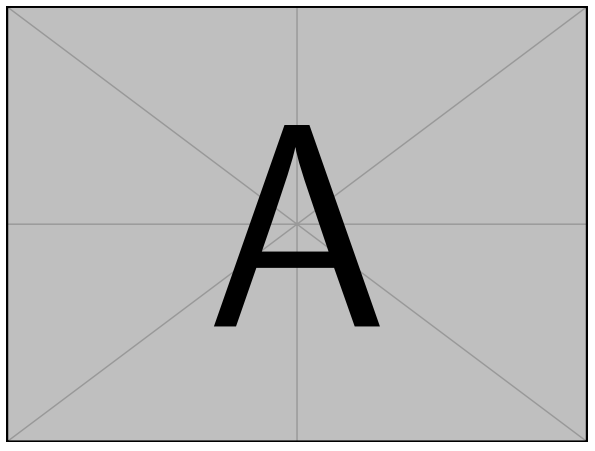
\includegraphics[width=\linewidth]{A (1).PNG}
        \caption{Output A}
        \label{fig:A}
    \end{subfigure}
    \hfill
    \begin{subfigure}{0.32\textwidth}
        \centering
        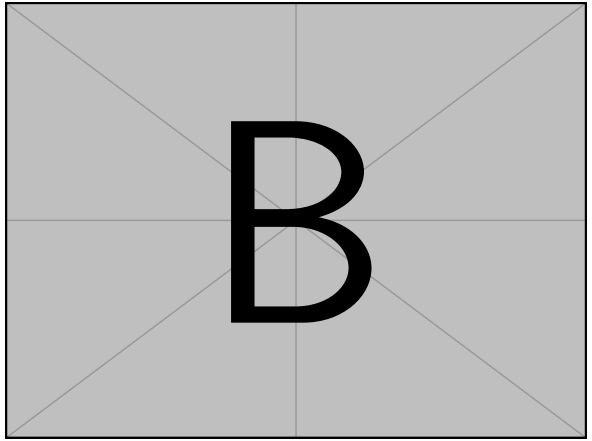
\includegraphics[width=\linewidth]{B (1).PNG}
        \caption{Output B}
        \label{fig:B}
    \end{subfigure}
    \hfill
    \begin{subfigure}{0.32\textwidth}
        \centering
        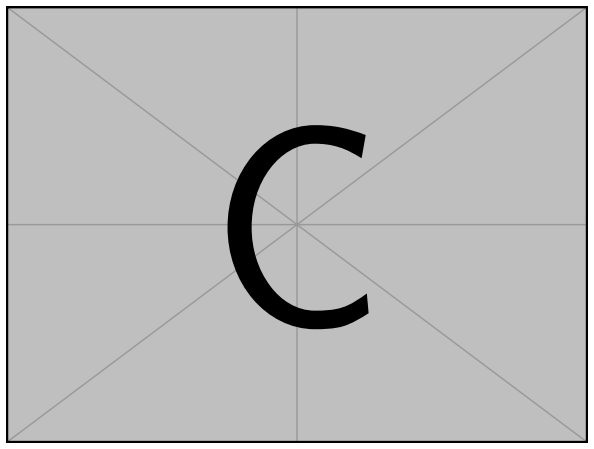
\includegraphics[width=\linewidth]{C (1).PNG}
        \caption{Output C}
        \label{fig:C}
    \end{subfigure}
    \caption{Comparison of three rendering outputs.}
    \label{fig:1}
\end{figure}
Figure 1 compares three different rendering outputs arranged in a single row.

\section{Conclusion}
Image synthesis combines \uline{mathematical precision}, algorithmic design, and efficient implementation. As scene complexity increases, choosing the appropriate
method becomes critical for balancing quality and performance.
\end{document}